\section{Prompts in Experienments}
\label{app:prompt}
We provide prompts for collecting teacher's responses in Figure~\ref{fig:gen_gsm8k} (GSM8K) and Figure~\ref{fig:gen_mmlu} (MMLU-PRO).

\begin{figure*}[!ht]
    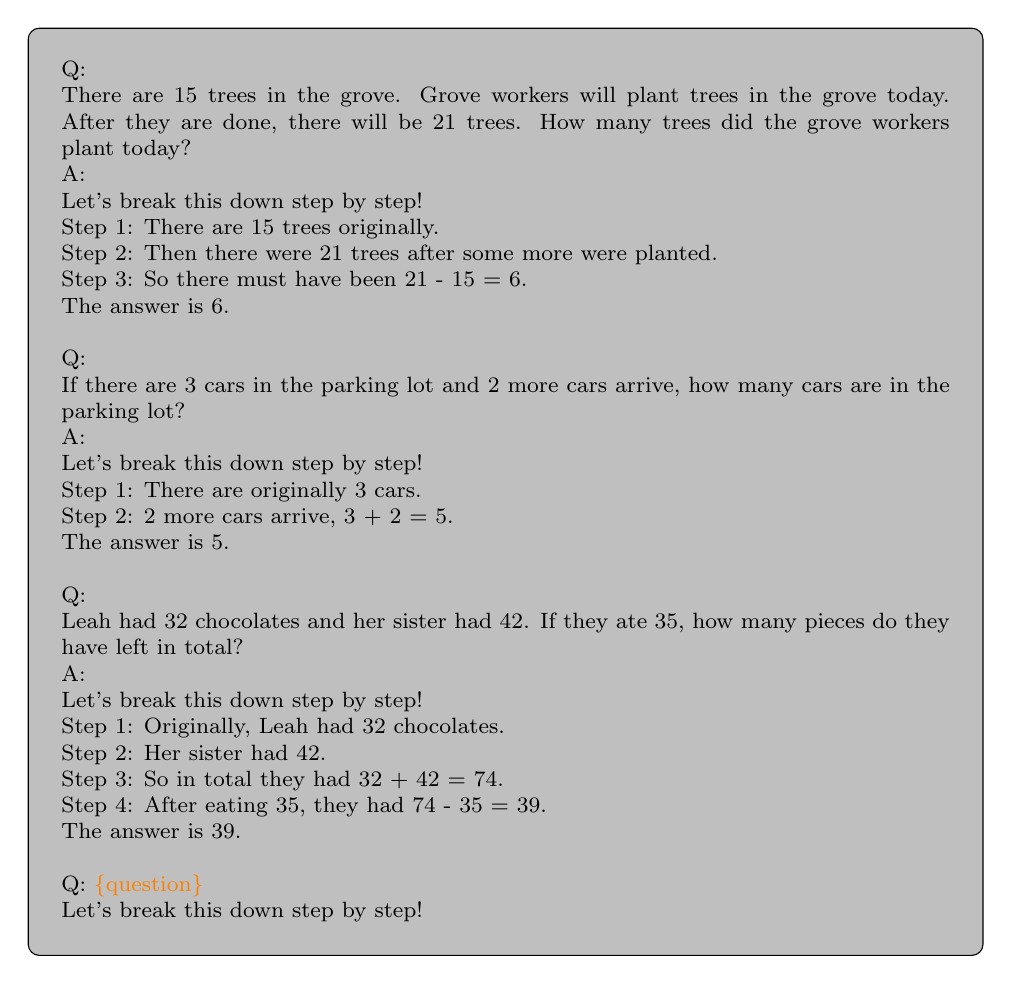
\begin{tikzpicture}
    \node [draw, rounded corners,
         text width=\linewidth-24pt,    % <---
         align=flush center, 
         inner sep=12 pt,
         fill=lightgray,
    ]%
    {
    \begin{minipage}{1\linewidth}
    \footnotesize{
Q: \\
There are 15 trees in the grove. Grove workers will plant trees in the grove today. After they are done, there will be 21 trees. How many trees did the grove workers plant today? \\
A: \\
Let's break this down step by step!\\
Step 1: There are 15 trees originally. \\
Step 2: Then there were 21 trees after some more were planted. \\
Step 3: So there must have been 21 - 15 = 6.\\
The answer is 6.\\

Q: \\
If there are 3 cars in the parking lot and 2 more cars arrive, how many cars are in the parking lot? \\
A: \\
Let's break this down step by step! \\
Step 1: There are originally 3 cars. \\
Step 2: 2 more cars arrive, 3 + 2 = 5. \\
The answer is 5.\\

Q: \\
Leah had 32 chocolates and her sister had 42. If they ate 35, how many pieces do they have left in total?\\
A: \\
Let's break this down step by step! \\
Step 1: Originally, Leah had 32 chocolates. \\
Step 2: Her sister had 42. \\
Step 3: So in total they had 32 + 42 = 74. \\
Step 4: After eating 35, they had 74 - 35 = 39. \\
The answer is 39.\\


Q: \color{orange}{\{question}\} } \\
Let's break this down step by step!
\end{minipage}
};
\end{tikzpicture}
\caption{
Prompt template for generating responses in the teacher LLMs over GSM8K dataset.
}
\label{fig:gen_gsm8k}
\end{figure*}


\begin{figure*}[!ht]
    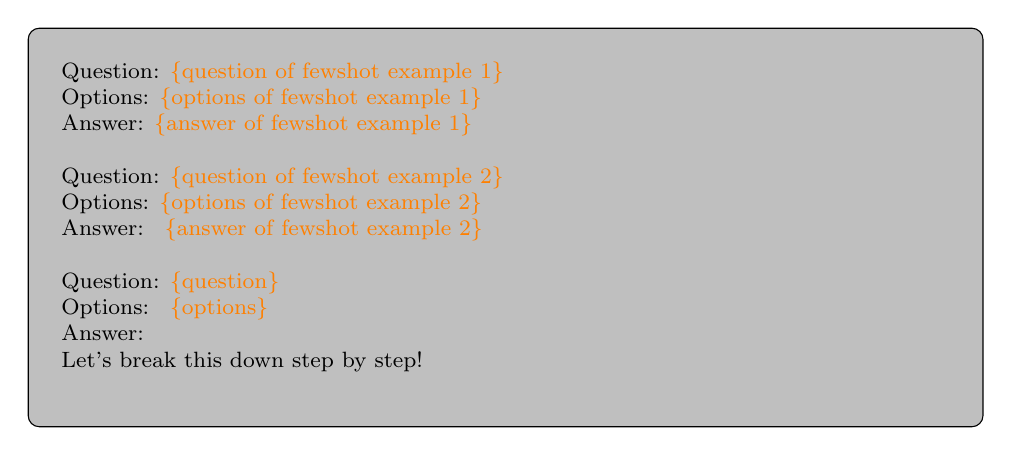
\begin{tikzpicture}
    \node [draw, rounded corners,
         text width=\linewidth-24pt,    % <---
         align=flush center, 
         inner sep=12 pt,
         fill=lightgray,
    ]%
    {
    \begin{minipage}{1\linewidth}
    \footnotesize{
Question:  {\color{orange}{\{question of fewshot example 1\}}} \\
Options: {\color{orange}{\{options of fewshot example 1\} }} \\
Answer: {\color{orange}{\{answer of fewshot example 1\} }} \\

Question:  {\color{orange}{\{question of fewshot example 2\} }} \\
Options: {\color{orange}{\{options of fewshot example 2\} }} \\
Answer: { \color{orange}{\{answer of fewshot example 2\} }}\\

Question: {\color{orange}{\{question\} }} \\
Options: { \color{orange}{\{options\}}}  \\
Answer: {} \\
Let's break this down step by step! }\\
\end{minipage}
};
\end{tikzpicture}
\caption{
Prompt template for generating responses in the teacher LLMs over MMLU-PRO dataset. We use two shots (provided by the dataset) for few-shot learning.
}
\label{fig:gen_mmlu}
\end{figure*}


\section{Implementation Details}
\subsection{Data Split}
\label{app:data_split}
For GSM8K, we divided the original training dataset into training and validation sets, allocating 90\% for training and 10\% for validation.

For MMLU-PRO, we first allocate 15\% of the data for testing. Then, we split the remaining data into training and validation sets using a 90\% to 10\% ratio.

\subsection{Hyperparameter}
\label{app:hyperparameters}
Our training pipeline consists of three stages: supervised fine-tuning (SFT) warm-up, reward model training, and proximal policy optimization (PPO). Each stage plays a critical role in progressively improving the student model.

\paragraph{Dataset Specific Hyper-parameters} We set the maximum generation length as $512$ for GSM8K and $1024$ for MMLU-PRO.
\paragraph{SFT Warm-up}

% Optimized Paragraph
The \textbf{Supervised Fine-Tuning (SFT)} phase serves to initialize the student model prior to reinforcement learning. During SFT, we employ a learning rate of \(5 \times 10^{-6}\) and a sequence length of 512 tokens. The batch size varies based on the specific teacher and student model configurations, as detailed in \textbf{Table \ref{tab:batch_sizes}}. Our dataset comprises majority-voted responses, ensuring a robust foundation for subsequent optimization. For the warm-up phase, we utilize 4 H100 GPUs and perform full parameter training. The training process spans 4 epochs, with checkpoints saved at intervals specified in the table. The optimal checkpoint is selected based on performance on the validation set. To accelerate training, we leverage DeepSpeed.

% Revised Table
\begin{table}[ht]
    \centering
    \begin{tabular}{ccccc}
        \toprule
        Dataset & Teacher Model & Student Model & Batch Size & Save Steps \\
        \midrule
        \multirow{4}{*}{GSM8K} 
            & \multirow{2}{*}{Llama3-70B} & Llama3-1B & 84 & 100 \\
            &                             & Llama3-3B & 74 & 100 \\ \cline{2-5}
            & \multirow{2}{*}{Llama3-8B} & Llama3-1B & 84 & 100 \\
            &                             & Llama3-3B & 70 & 100 \\
        \midrule
        \multirow{4}{*}{MMLU-PRO} 
            & \multirow{2}{*}{Llama3-70B} & Llama3-1B & 40 & 400 \\
            &                             & Llama3-3B & 32 & 400 \\ \cline{2-5}
            & \multirow{2}{*}{Llama3-8B} & Llama3-1B & 40 & 100 \\
            &                             & Llama3-3B & 32 & 100 \\
        \bottomrule
    \end{tabular}
    \caption{Batch size and checkpoint saving steps in warm up phase.}
    \label{tab:batch_sizes}
\end{table}



\paragraph{Reward Model Training}
The reward model is trained to guide PPO-based fine-tuning. This stage uses a learning rate of $5\times10^{-5}$, a batch size of 48 for student Llama3-1B and a batch size of 16 for student Llama3-3B, and 4 training epochs. We apply early stop while the reward model performance stop increasing on validation set.The reward model is initialized from the student model after warm up.
All reward models were trained on four H100 GPUs.

\paragraph{PPO Training}
The PPO stage refines the student model through reinforcement learning with the reward model. We use a learning rate of $1\times10^{-5}$, a KL penalty coefficient of 0.2, and a value function coefficient of 0.1. The total number of training episodes is set to $200,000$, ensuring sufficient interaction with the reward model for stable policy improvement. We apply early stop while the student model performance stop increasing on validation set. We present more hyper-parameters in Table~\ref{tab:batch_sizes_ppo}.

\begin{table}[ht]
    \centering
    \begin{tabular}{cccccc}
        \toprule
        Dataset & Teacher Model & Student Model & Batch Size & Learning Rate & GPU\_NUM\\
        \midrule
        \multirow{4}{*}{GSM8K} 
            & \multirow{2}{*}{Llama3-70B} & Llama3-1B & 20 & $1\times 10^{-5}$ & 2\\
            &                             & Llama3-3B & 4 & $5\times 10^{-6}$  & 4\\
            & \multirow{2}{*}{Llama3-8B} & Llama3-1B & 20 & $1\times 10^{-5}$  & 2\\
            &                             & Llama3-3B & 4 & $5\times 10^{-6}$  & 4\\
        \midrule
        \multirow{4}{*}{MMLU-PRO} 
            & \multirow{2}{*}{Llama3-70B} & Llama3-1B & 10 & $5\times10^{-6}$ &  4 \\
            &                             & Llama3-3B & 2 & $1\times10^{-5}$ & 4 \\
            & \multirow{2}{*}{Llama3-8B} & Llama3-1B & 10 & $1\times10^{-5}$  & 4 \\
            &                             & Llama3-3B & 2 & $1\times10^{-5}$  & 4  \\
        \bottomrule
    \end{tabular}
    \caption{Hyper-parameters in PPO.}
    \label{tab:batch_sizes_ppo}
\end{table}

\paragraph{\textbf{Ours w/o Data}} We apply a learning rate of $5\times^10{-5}$ and KL coefficient of 0.1 in this ablation version. Other hyper-parameters are the same to \textbf{PPO Training}.


